\fuxiti
\begin{xiaotis}

\xiaoti{已知: $\triangle ABC$ 的中线 $AD$、$BE$ 交于点 $G$。
    求证: $S_{\triangle ABG} = S_{\text{四边形} CEGD}$。
}


\xiaoti{求证:梯形面积等于一腰和另一腰中点到这个腰的距离的积。}

\xiaoti{把一个已知梯形改成和它面积相等的等腰梯形,使它两底的大小不变。}

\xiaoti{图中两块土地之间有一条小路 $CFG$,用作图方法把它改成经过点 $C$ 的直路。
    使路两旁的土地面积不变。
}

\begin{figure}[htbp]
    \centering
    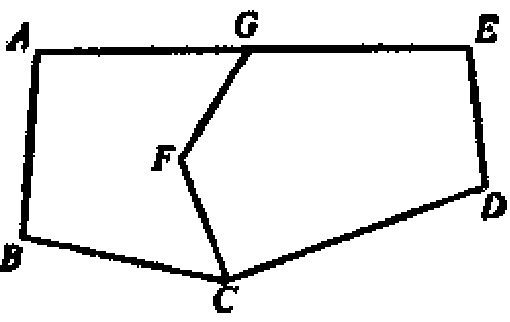
\includegraphics[width=5.0cm]{../pic/czjh1-ch5-fuxi-04.png}
    \caption*{(第 4 题)}
\end{figure}


\xiaoti{三边长为 $2n^2 + 2n$, $2n+1$, $2n^2 + 2n + 1 \; (n > 0)$ 的三角形
    是不是直角三角形?为什么?
}

\xiaoti{一个直角三角形的三边为三个连续整数,求它各边的长。}

\xiaoti{一个等腰三角形底边和腰的长分别为 12 厘米和 10 厘米。
    有一矩形,它的周长和面积与这个等腰三角形的周长和面积分别相等。
    求矩形的长与宽。
}

\xiaoti{}%
\begin{xiaoxiaotis}%
    \xxt[\xxtsep]{已知: $\triangle ABC$ 的 $\angle A : \angle B : \angle C = 1:2:3$。
        求证: $b^2 = 3a^2$。
    }

    \xxt{已知: $\triangle ABC$ 的 $\angle A : \angle B : \angle C = 1:1:2$。
        求证: $c^2 = 2a^2$。
    }

\end{xiaoxiaotis}

\xiaoti{已知: 在 $\triangle ABC$ 中, $\angle C = Rt \angle$, $CD$ 是高。
    求证: $2 CD^2 + AD^2 + BD^2 = AB^2$。
}

\xiaoti{在 $\triangle ABC$ 中, $AB > AC$, $AD$ 是中线, $AE$ 是高。
    求证: $AB^2 - AC^2 = 2 BC \cdot DE$。
}

\xiaoti{已知菱形的周长是 52 cm, 一条对角线长是 24 cm。
    求它的面积。
}

\xiaoti{求证:菱形的对角线的平方和等于一边平方的 4 倍。}

\xiaoti{用一条 36 寸长的铁丝弯成一个直角三角形的模型,
    要使它的一条直角边比另一条直角边短 3 寸。 应该怎样弯。
}

\end{xiaotis}

